
%User Manual
%\chapter{User Manual}
 \chapter{Manual utilizator}

\label{cap:user-manual}
%
%Descrie pașii de instalare și rulare a aplicației. Dacă dezvoltarea aplicației s-a bazat sau a presupus instalarea și configurarea unei infrastructuri (complexe), descrieți detaliat pașii pe care i-ați urmat (referințele utilizate) și mai ales abaterile voite sau necesare de la documenațiile referite. Încercați ca cineva care vă continuă tema să nu mai fie nevoit să mai piardă timp inutil cu pregătirea mediului de lucru și să poată trece cât mai repede la abordarea temei proptriu-zise a proiectului. 
%
%Indincați, de asemenea, explicit versiunile aplicațiilor, bibliotecilor folosite și salvați o copie a acestora pe CD-ul atașat lucrării. E posibil ca aplicația voastră să nu mai funcționeze la fel pe alte versiuni și e bine de știut acest lucru și,  în același timp, e bine ca mediul descris de voi să poată fi reprodus ulterior. 
%
%Se întinde pe aproximativ 2-3 pagini. 

\section{Instalarea proiectului}

Pentru instalarea sistemului, atât timp cât toate dependințele acestuia sunt împlinite, utilizatorul nu mai trebuie să facă nimic. Toate fișierele necesare sistemului au fost împachetate în modulul principal, singurul pas ce poate fi executat de utilizator este crearea unui shortcut către executabilul ce lansează în execuție sistemul. 
\section{Utilizare}

După deschiderea aplicației, utilizatorul este întâmpinat de meniul de Home al acesteia. În următoarea fereastră se poate observa designul acestuia:  

\begin{figure}[h]
	\centering
	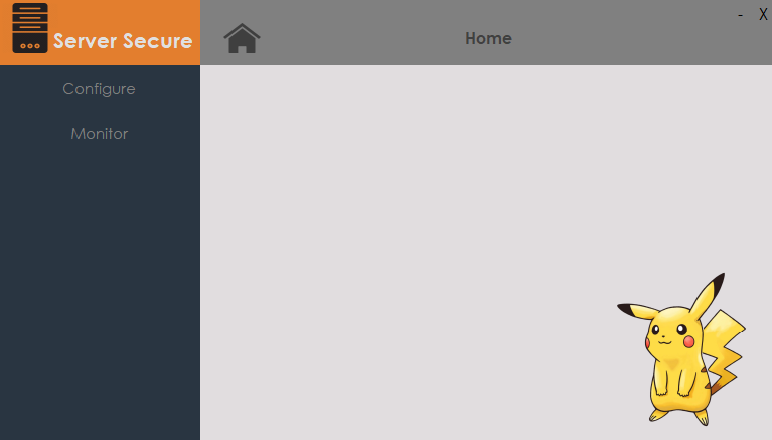
\includegraphics[width=0.6\textwidth]{ui_home.png}
	\caption{ Meniul "Home" în interfața grafică }
	\label{fig:ui_home}
\end{figure}

În partea superioară a ferestrei se află în permanență numele ferestrei curente(în cazul de față fereastra Home). În meniul prezent în stânga ferestrei sunt situate celelate două ferestre disponibile utilizatorului: Configure și Monitor. Utilizatorul poate să navighze între aceste ferestre dând un click pe numele ferestrelor, respectiv pe pictograma în formă de căsuță pentru meniul Home.  \\

\begin{figure}[h]
	\centering
	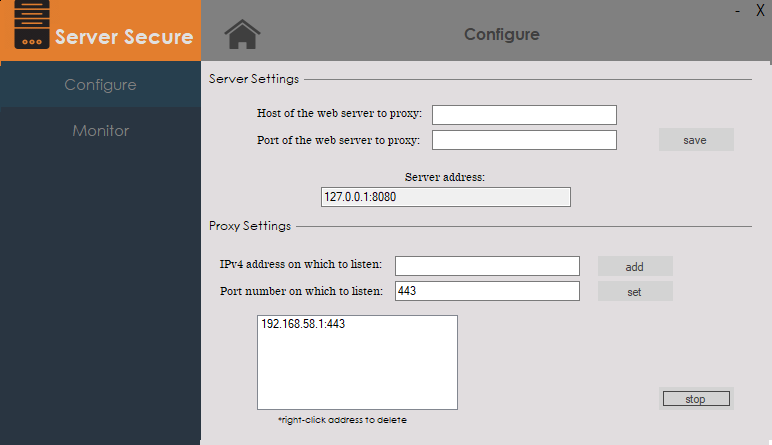
\includegraphics[width=0.7\textwidth]{ui_configure.png}
	\caption{ Meniul "Configure" în interfața grafică }
	\label{fig:ui_configure}
\end{figure}

În fereasra Configure, utilizatorul poate să seteze parametrii de rulare a sistemului. Acestuia i se prezintă două rubrici: Server Settings și Proxy Settings. În partea de Server Settings, utilizatorul setează datele server-ului: adresa IP a acestuia și portul aferent pe care acesta acceptă conexiunui. Salavarea sau suprascrierea acestor date se realizează prin apăsarea butonului "save" din rubrica respectivă. În partea de Proxy Settings, utilizatorul poate să introducă mai multe adrese IP și un port, pe care sistemul să accepte conexiuni și să le redirectioneze către server. După setarea parametrilor de mai sus, sistemul se poate porni/opri prin apăsarea butonului din dreapta jos(cu textul "start"/"stop" după caz). 
\newpage
\begin{figure}[h]
	\centering
	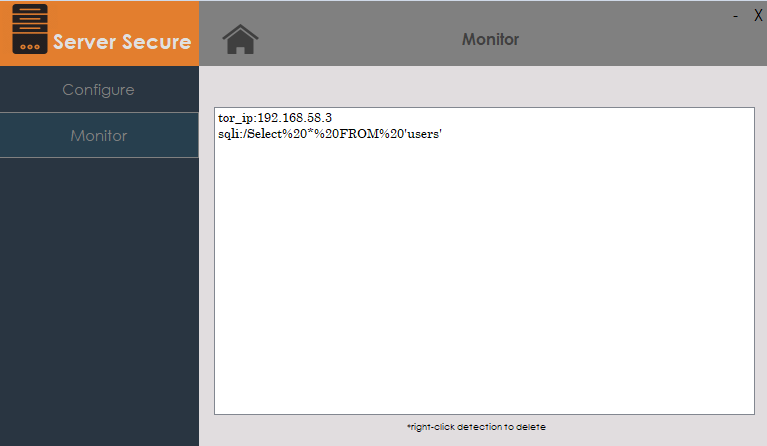
\includegraphics[width=0.8\textwidth]{ui_monitor.png}
	\caption{ Meniul "Monitor" în interfața grafică }
	\label{fig:ui_monitor}
\end{figure}

În fereastra de Monitor, utilizatorul poate să urmărească activitatea sistemului. În cazul în care sistemul detectează un eveniment, acesta este afișat în interfața grafică în această fereastre(conform exemplului din imagine). Dacă utilizatorul dorește ștergerea evenimentelor antrioare, aceasta se poate realiza prin click dreapta pe eveniment. 